\subsection{Development of the LHC-MKI Beam Screen}
\label{sec:mki-screen-development}

Concerns about the beam coupling impedance of the SPS extraction kicker magnets (MKEs), and thus beam induced heating with LHC type beam with high current, led to detailed investigation of the SPS kicker magnets \cite{Arduini:beamInducedSPS}. During an extensive measurement campaign, it was deduced that extensive beam-induced heating was due to the large real component of the longitudinal impedance of the MKEs. Subsequently a number of retroactive impedance reduction methods were proposed and evaluated for their effectiveness in decreasing the longitudinal impedance \cite{Kroyer:MKEReduct}.

There had previously been debate on the need for a beam screen for the LHC-MKIs \cite{Vos:beamScreen}: however the beam screen was considered early in the design \cite{Ducimetiere:designMKI}, which ultimately was implemented in the final design \cite{Barnes:improvBeamScreen}. The beam screen is composed of a ceramic tube housing up to 24 screen conductors - conductive wires which extend beyond the length of the ferrite yoke, connected directly to the LHC beam pipe at one end, and capacitively coupled to it at the other. A scheme involving printed conductive strips on the inside surface of the ceramic was tested but was not implemented due to extensive surface electrical breakdown between the strips during pulsing of the kickers. The capacitive coupling is required due to the short rise time requirement of the kicker field - direct connections at both ends would create a short-circuit secondary, causing the characteristic rise time of the system to dramatically increase. In this case electrical simulations indicate that the optimum is with the capacitive coupling at the pulse input end, i.e. the upstream end of the kicker \cite{Barnes:improvBeamScreen}. This will become relevant during the evaluation of heating patterns of the MKI during operation.

The use of the capactive coupling gives rise to a discontinuity of the conducting path of the beam image current. This results in the possibility of exciting resonances in the surrounding structure of the image current path. In this case, resonant modes of a characteristic frequency due to the screen conductors acting as $n \lambda /4$ resonators. To damp these low frequency modes (the screen conductors are some 3m in length), nine ferrite (NiZn) toroids are placed at each end of the beam screen \cite{Caspers:impMeasMKI, Caspera:impMeasLowFreqMKI, Barnes:mkiVacTemp}. Cross sections of the beam screen are shown in Fig.~\ref{fig:beamScreenCross} for clarity.

During testing and conditioning of the MKIs it was discovered than there was still significant surface electrical breakdown/sparking occuring on the outside surface of the ceramic tube during pulsing. Measurements showed that above a PFN voltage of 30kV large quantities of discharge were observed originating from the screen conductors. In particular, the highest induced voltage was known to occur on the screen conductors closest to the HV busbar \cite{Barnes:improvBeamScreen}. Due to the operational voltage requirements, and as it is not feasible to operate the kicker magnets with a PFN voltage below approximately 51kV, a solution had to be found. Following detailed electromagnetic simulations it was decided to remove the screen conductors with the highest induced voltages (those closest to the HV busbar) in an effort to reduce the number of discharges. Removing the 9 screen conductors closest to the HV busbar increased the PFN voltage reached, before discharges began, to 57kV, above the required 54kV to meet the design parameters for the MKI. Measurements demonstrated that this would worsen the longitudinal beam coupling impedance but this was determined to not be large enough to pose a problem from the point of view of beam induced heating \cite{Barnes:improvBeamScreen}.

\begin{figure}
\subfigure[]{
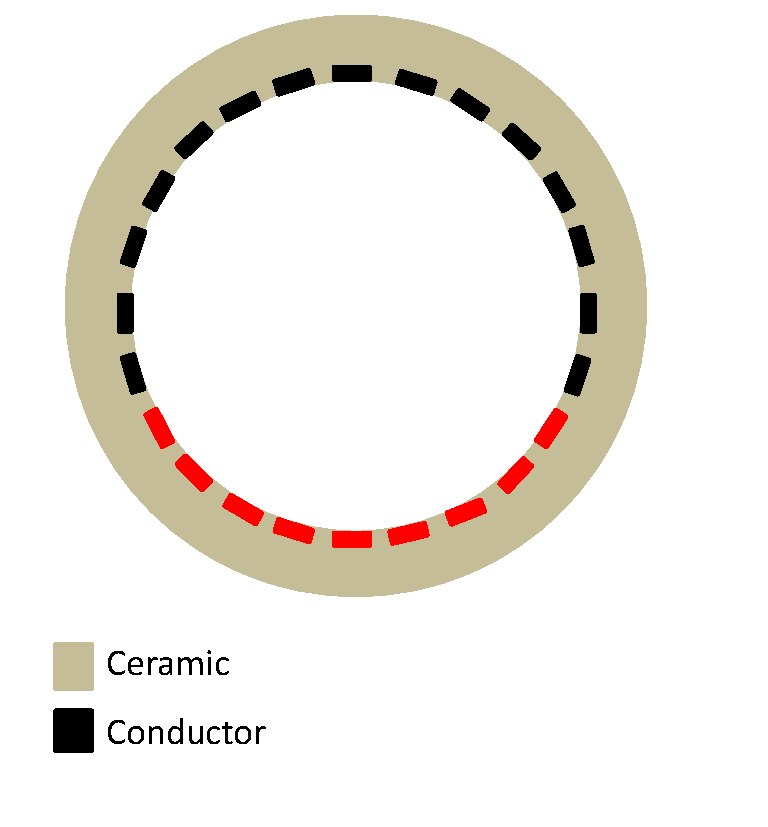
\includegraphics[width=0.3\textwidth]{LHC_MKI/figures/cross_section.pdf}
\label{fig:mkiCrossSec}
}
\subfigure[]{
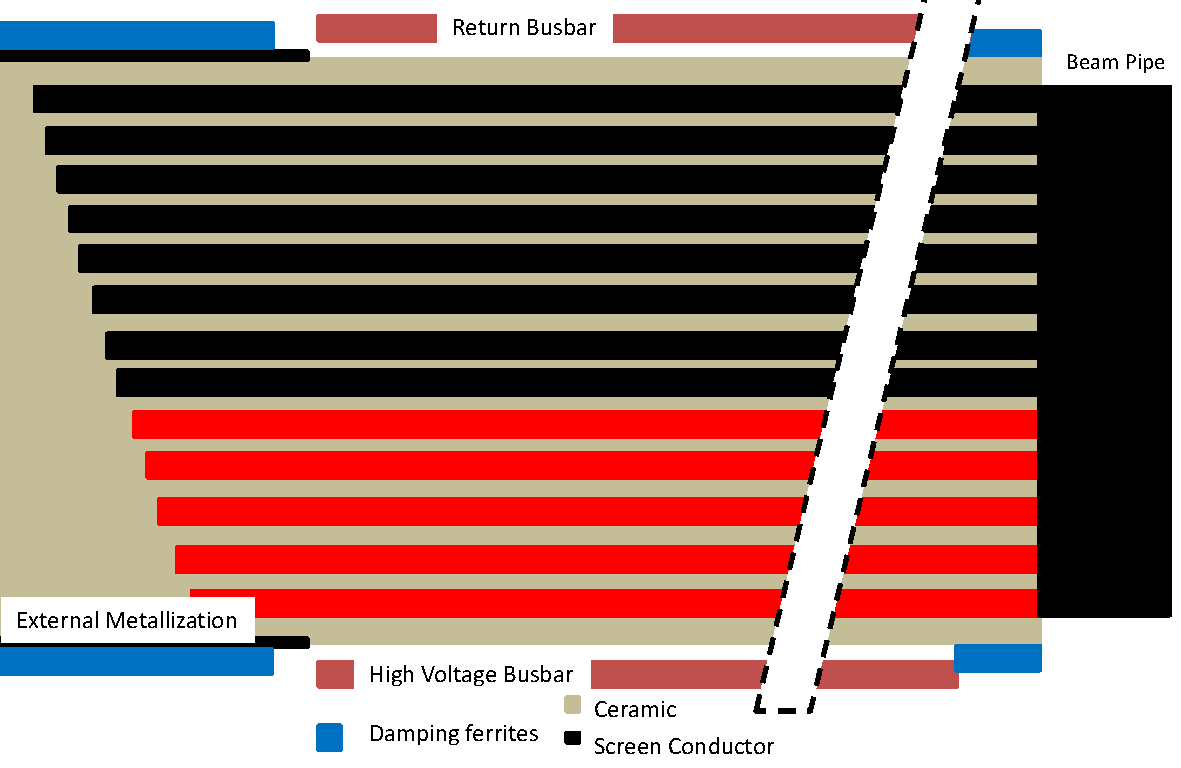
\includegraphics[width=0.7\textwidth]{LHC_MKI/figures/beamScreenCapEnd.pdf}
\label{fig:beamScreenCapEnd}
}
\caption{Cross sections of the beam screen perpendicular to \subref{fig:mkiCrossSec} and parallel to \subref{fig:beamScreenCapEnd} the direction of beam travel. The screen conductors removed from the majority of the MKIs during the original construction phase are highlighted in red.}
\label{fig:beamScreenCross}
\end{figure}

\subsection{Observations of heating during 2011 and 2012 until Technical Stop 3 (23.09.2012 - 27.09.2012)}

Beginning with the increasing intensity in the LHC during operation in 2011 a number of devices within the LHC were observed to be heating \cite{ Salvant:Heating, Metral:Heating}. Observations and calculations demonstrated a strong relationship between the observed heating and the increasing intensity (first the number of bunches, then the increase in bunch population) indicating that the source of the heating was due to the stored beam interacting strongly with the impedance of many structures - evidenced also by the deteriorating vacuum in some components also. A number of key devices were observed to be exposed to significant heating, in particular devices around the injection region (injection protection collimators, injection kickers, VMTSA (a two beam vacuum interconnect in the injection region in which two beams circulate) and some small insertion devices (ALFA roman pot), as explained at the workshops in Evian in 2011 \cite{Salvant:Heating} and Chamonix 2012 \cite{Metral:Heating}. 

Four PT-100 thermocouples are used for measuring temperatures in each MKI tank, the locations of which are shown in Fig.~\ref{fig:mkiCrossSectionYZ}. The purpose of these PT-100s is to give an indication of the temperature of the ferrite yoke and also of the temperature of the ferrite toroids. Ideally the 2 PT-100s used to indicate the temperature of the ferrite yoke woud be directly in thermal contact with the ferrite; however this is not possible as the ferrite is also pulsed to high voltages. Thus, instead, these two PT-100s are connected to the outermost ground plates, up and down stream. Thus the temperatures measured using these two PT-100s read lower than the actual ferrite yoke temperature. In addition since the magnet is in high vacuum, heat transfer between the different parts of the magnet is not well defined due to the lack of heat transfer via convection, and the complex transfer of heat by conduction and radiation within the magnet structure.

The measured heating of the LHC-MKIs in particular is shown in Fig.~\ref{fig:mki-heating-2011}. Some important notes about the heating can be made, firstly that MKIs 8b and 8d both show high measured temperatures, MKI8d in particular demonstrating much higher measured temperatures, showing temperatures $\approx$20$^{\circ}$C higher than that experienced by the other MKIs. Secondly, that the cooling time to return below the interlock temperature is very long (on the order of 4 hours \cite{Goddard:timeConst}), indicating a large portion of the ferrite yoke is heating, and additionally that the temperature reached was detrimental to magnet operation (i.e. the ferrite yoke was above it's Curie temperature, thus the magnetic field quality was not suitable for injection), hence the necessary cool-down time was substantial enough to affect machine operational schedules. It can also be seen that the peak temperature only gets worse as the beam intensity is increased.

\begin{figure}
\begin{center}\subfigure[]{
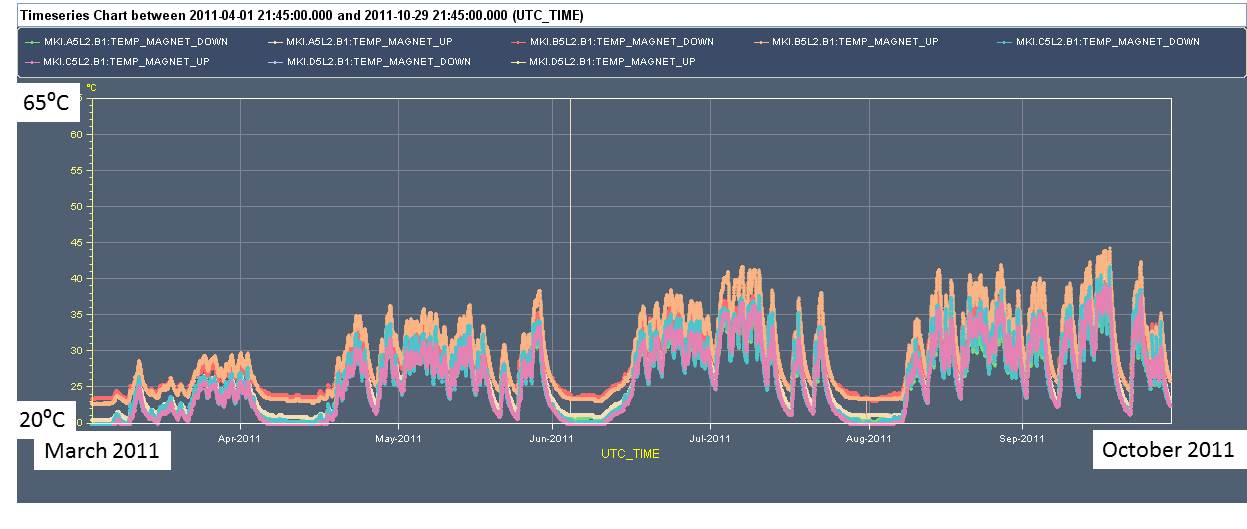
\includegraphics[width=1.0\textwidth]{LHC_MKI/figures/mkipt2HeatingBefore.jpg}
\label{fig:mki-ip2-heating-2011}
}
\subfigure[]{
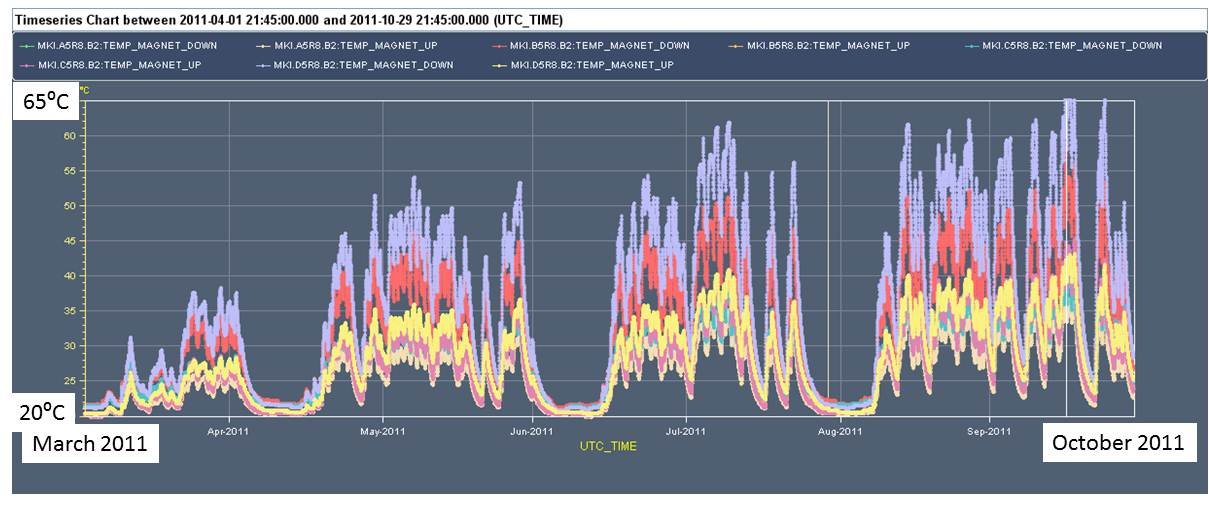
\includegraphics[width=1.0\textwidth]{LHC_MKI/figures/mkipt8HeatingBefore.jpg}
\label{fig:mki-ip8-heating-2011}
}
\end{center}
\caption{The measured temperature of the MKIs at \subref{fig:mki-ip2-heating-2011} IP2 and \subref{fig:mki-ip8-heating-2011} IP8 during 2011 in the LHC. Note MKI8b and MKI8d show significantly higher measured temperatures than the other MKIs.}
\label{fig:mki-heating-2011}
\end{figure}

The temperature of concern in the MKI is that of the ferrite yoke - to ensure that it is below the Curie point - but as mentioned above there are no direct temperature measurement on this component, hence one difficulty in analysing the heating of the MKI is to identify the actual temperature of the ferrite yoke corresponding to the measured temperature. This is a problem which has been analysed in depth in \cite{Barnes:mkiHeating}, in particular inferring the inductance of the magnet under a softstart condition (the pulsing of the magnet with no beam to inject). The softstart is carried out very soon after a beam dump when the ferrite yoke is at its highest temperature. Hence this analysis gives a certain margin of safety to the interlock level, but due to the possible damage that may be done due to a misinjection of the beam a conservative approach is necessary. Thus a few hours of cool down time between injections may still be required.

Prior to technical stop 3 in 2012 there were 2 configurations of the beam screen in the LHC-MKIs - 7 MKIs were in place with 15 (some staggered, some tapered) screen conductors, the 9 screen conductors closest to the HV busbar having been removed due to the electrical breakdown concerns mentioned in Sec.~\ref{sec:mki-screen-development} \cite{Barnes:improvBeamScreen}. A single MKI, MKI8c, was fitted with 24 screen conductors, 15 tapered and 9 shortened screen conductors (trimmed such they do not overlap with the external metallization at the capacitively coupled end). This was to reduce the electric field at the end of the screen conductors closest to the HV busbar, but not significantly improve the beam coupling impedance of the MKI \cite{Barnes:improvBeamScreen}.